% !TEX root = ../ausarbeitung.tex

\chapter{Evaluation}

Die Applikation wurde mit dem Hauptziel entwickelt, eine Nutzeroberfläche zu entwickeln, mit der sowohl Personen, die in der LRS Therapie arbeiten (wie Lerntherapeuten oder Nachhilfelehrer) als auch Nicht-Experten (z.B. die Eltern betroffener Kinder) intuitiv und effizient benötigtes Arbeitsmaterial erstellen können. Außerdem wurde untersucht wie eine Datenbank für Betonungsmuster in Wörtern erstellt und benutzerfreundlich erweitert werden kann.\\

Die Evaluation untersucht daher folgende Punkte:
\begin{itemize}
	\item Erstellung von Arbeitsmaterial aus einem einfachen Text 
	\item Intuitivität und Einfachheit der Bedienung
	\item Effizienz des Prozesses der Erstellung von Arbeitsmaterial
	\item Unterschiede in der Bedienung durch Experten und Laien
	\item Nutzerfreundliche Erweiterung der Wortdatenbank
\end{itemize}

Zunächst wird durch Beispiele eines annotieren Textes mit verschiedenen Einstellungen demonstriert, welche vielseitigen Möglichkeiten die Textannotation für das Erstellen von Arbeitsmaterial bietet. Für die Untersuchung von Intuitivität, Einfachheit und Effizienz bei der Bedienung der Applikation wurde ein Nutzertest durchgeführt. Dieser fand als Interview statt um qualitative Daten durch Nutzerbefragung zu erheben. Außerdem wurden quantitative Daten durch das Ausfüllen von Ankreuzfragen während des Interview erhoben.

\section{Ergebnisse der Textannotation}
\label{sec:annotation-results}

Um zu zeigen, dass die Applikation das Ziel des automatischen Erstellens von Arbeitsmaterial erfüllt, werden im Folgenden verschiedene Texte präsentiert, die mit Hilfe des Web Interfaces erstellt wurden. Die Ergebnisse zeigen, dass das Programm diese Ziel nicht nur erfüllt, sondern im Vergleich zu herkömmlichen Methoden \tocite{Silbefibel, ABC} auch noch einen hohen Grad an Flexibilität bietet. Die Einstellungen und damit das Erscheinungsbild des resultierenden Textes können vom Nutzer frei an die Bedürfnisse des jeweiligen Falls angepasst werden.\\

Im Folgenden wurde der Beispieltext \textit{Aschenputtel} mit der Web Applikation analysiert, sodass Silbentrennung und Betonung farblich markiert dargestellt werden. Die in den Beispielen verwendeten Texten wurden mit der Druckfunktion der Textvorschau als PDF Dateien exportiert. Jedes Bild entspricht einer DIN A4 Seite.

\subsubsection{Beispiel 1: Hervorhebung der Silben mit zwei alterierenden Farben}

Im ersten Beispiel wird die Schriftfarbe für da Hervorheben der Silben genutzt. Die betonte Silbe wird immer rot dargestellt, in Wörtern mit vielen Silben, werden diese dann alterierend rot und blau hervorgehoben. Die Schriftgröße wurde auf \textit{22} gesetzt, der Wortabstand auf den Wert \textit{0.4}. Zusätzlich sorgt die Einstellung des Zeilenabstands auf \textit{1.5} für bessere Lesbarkeit.

\begin{figure}[h!]
	\centering
	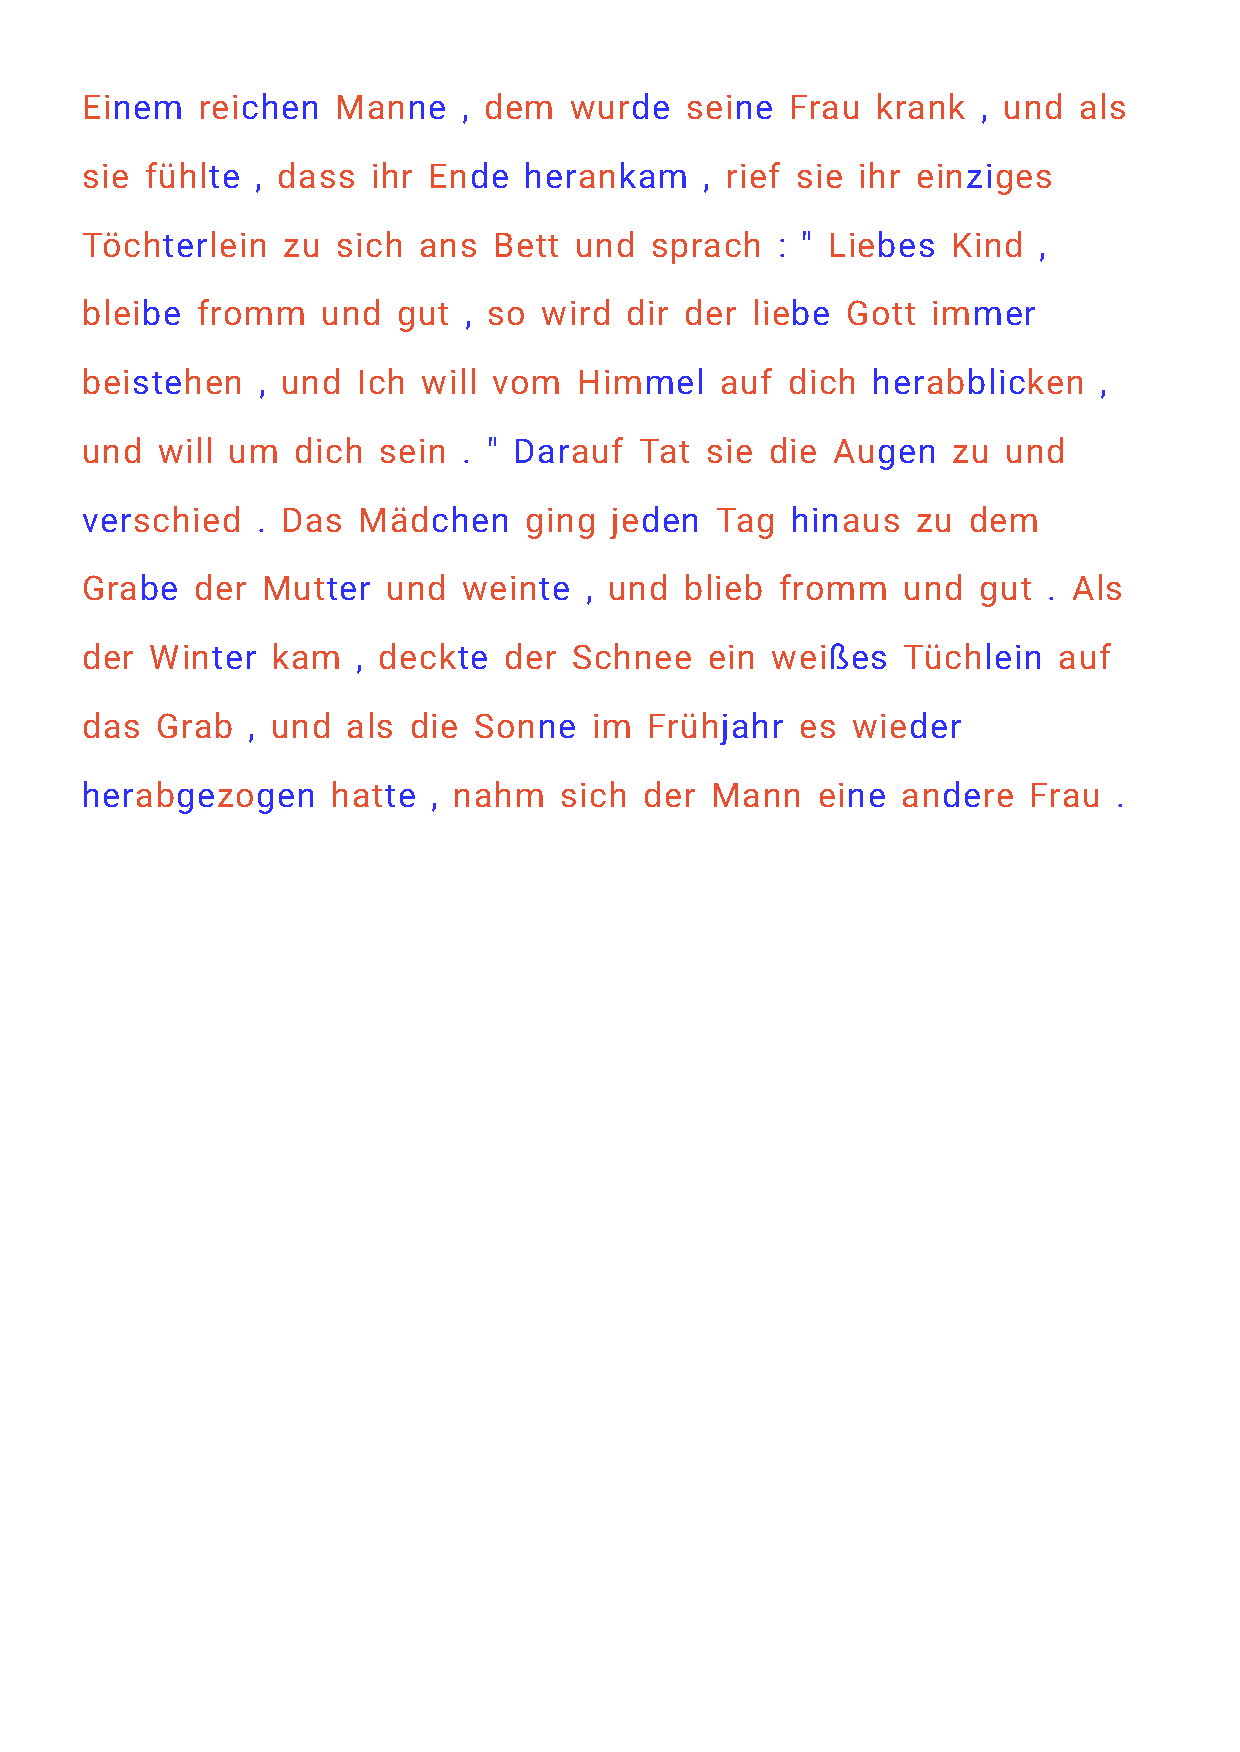
\includegraphics[width=.7\linewidth, frame]{figures/evaluation/annotation1}
	\caption{Hervorhebung der Silben mit zwei alterierenden Farben}
	\label{fig:evaluation-ex1}
\end{figure}
\newpage

\subsubsection{Beispiel 2: Worthintergrund und Silbenabstand}

In diesem Beispiel sorgt die Worthintergrundfarbe für eine bessere Wahrnehmung des Wortes als Einheit. Dadurch kann auch ein Silbenabstand (hier \textit{0.1}) eingestellt werden ohne dass die Gefahr besteht, dass dadurch nicht mehr klar ist, welche Silben zusammen gehören. Wegen dem Worthintergrund nehmen die Wörter mehr Platz in der Zeile ein, daher wurde auch der Zeilenabstand auf \textit{2.2} erhöht. Zudem wurde hier ein Zeichenabstand von \textit{2} (statt \textit{1} in Beispiel 1) gewählt.

\begin{figure}[h!]
	\centering
	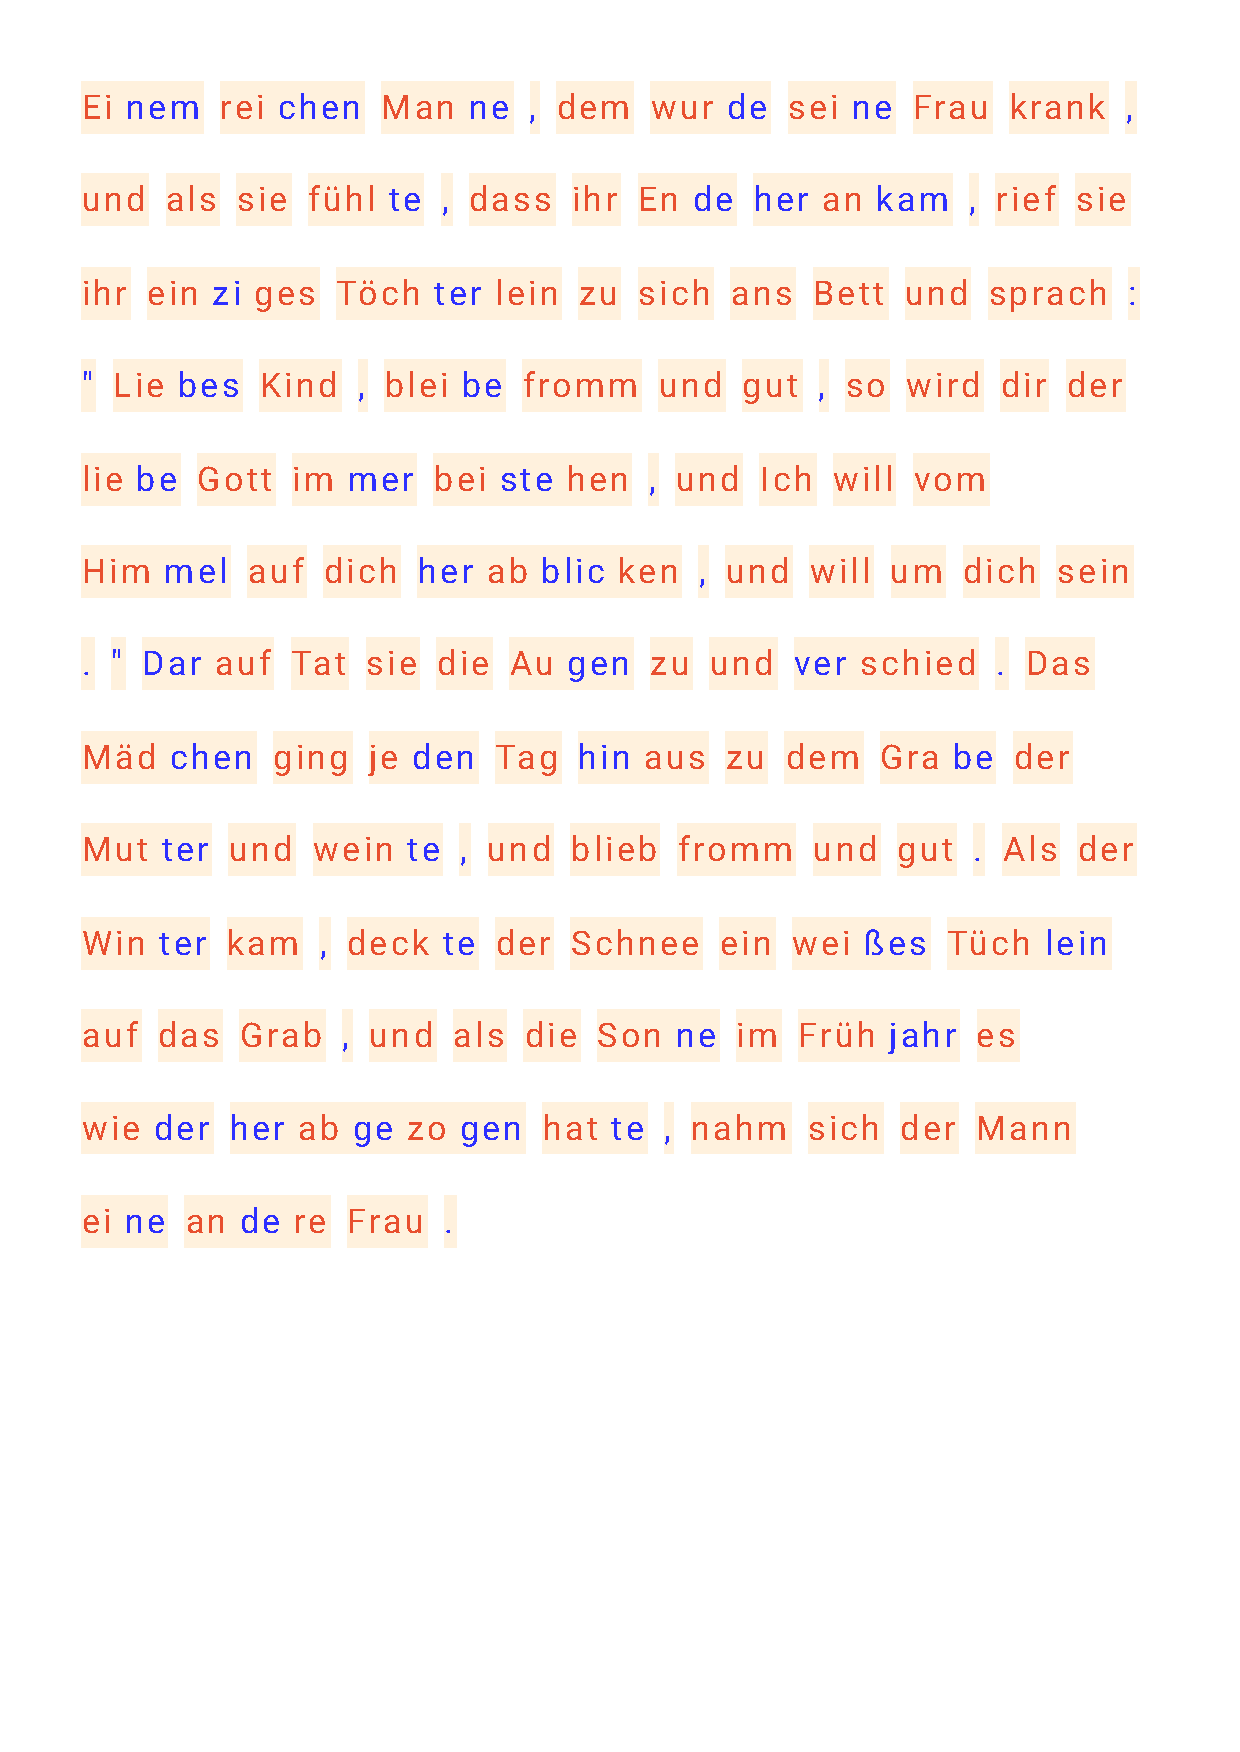
\includegraphics[width=.7\linewidth, frame]{figures/evaluation/annotation2}
	\caption{Worthintergrund und Silbenabstand}
	\label{fig:evaluation-ex2}
\end{figure}
\newpage

\subsubsection{Beispiel 3:  Silbentrennzeichen und verschiedene Silbenfarben}

In Beispiel 3 wurde wieder auf die Worthintergrundfarbe verzichtet. Das Trennzeichen \qq{=} soll hier das Silbentrennen erleichtern, sowie zusammenhängende Silben zu einem Wort gruppieren. Der Zeichenabstand beträgt wieder \textit{1}, der Silbenabstand \textit{0}, da das Gleichheitszeichen hier als Silbentrenner dient. Zusätzlich wurde eine weitere Farbe für alterierende Silben gewählt. Hier wird nur noch die betonte Silbe rot dargestellt, danach alterieren die Silben bei langen Wörtern in den Farben blau und lila.

\begin{figure}[h!]
	\centering
	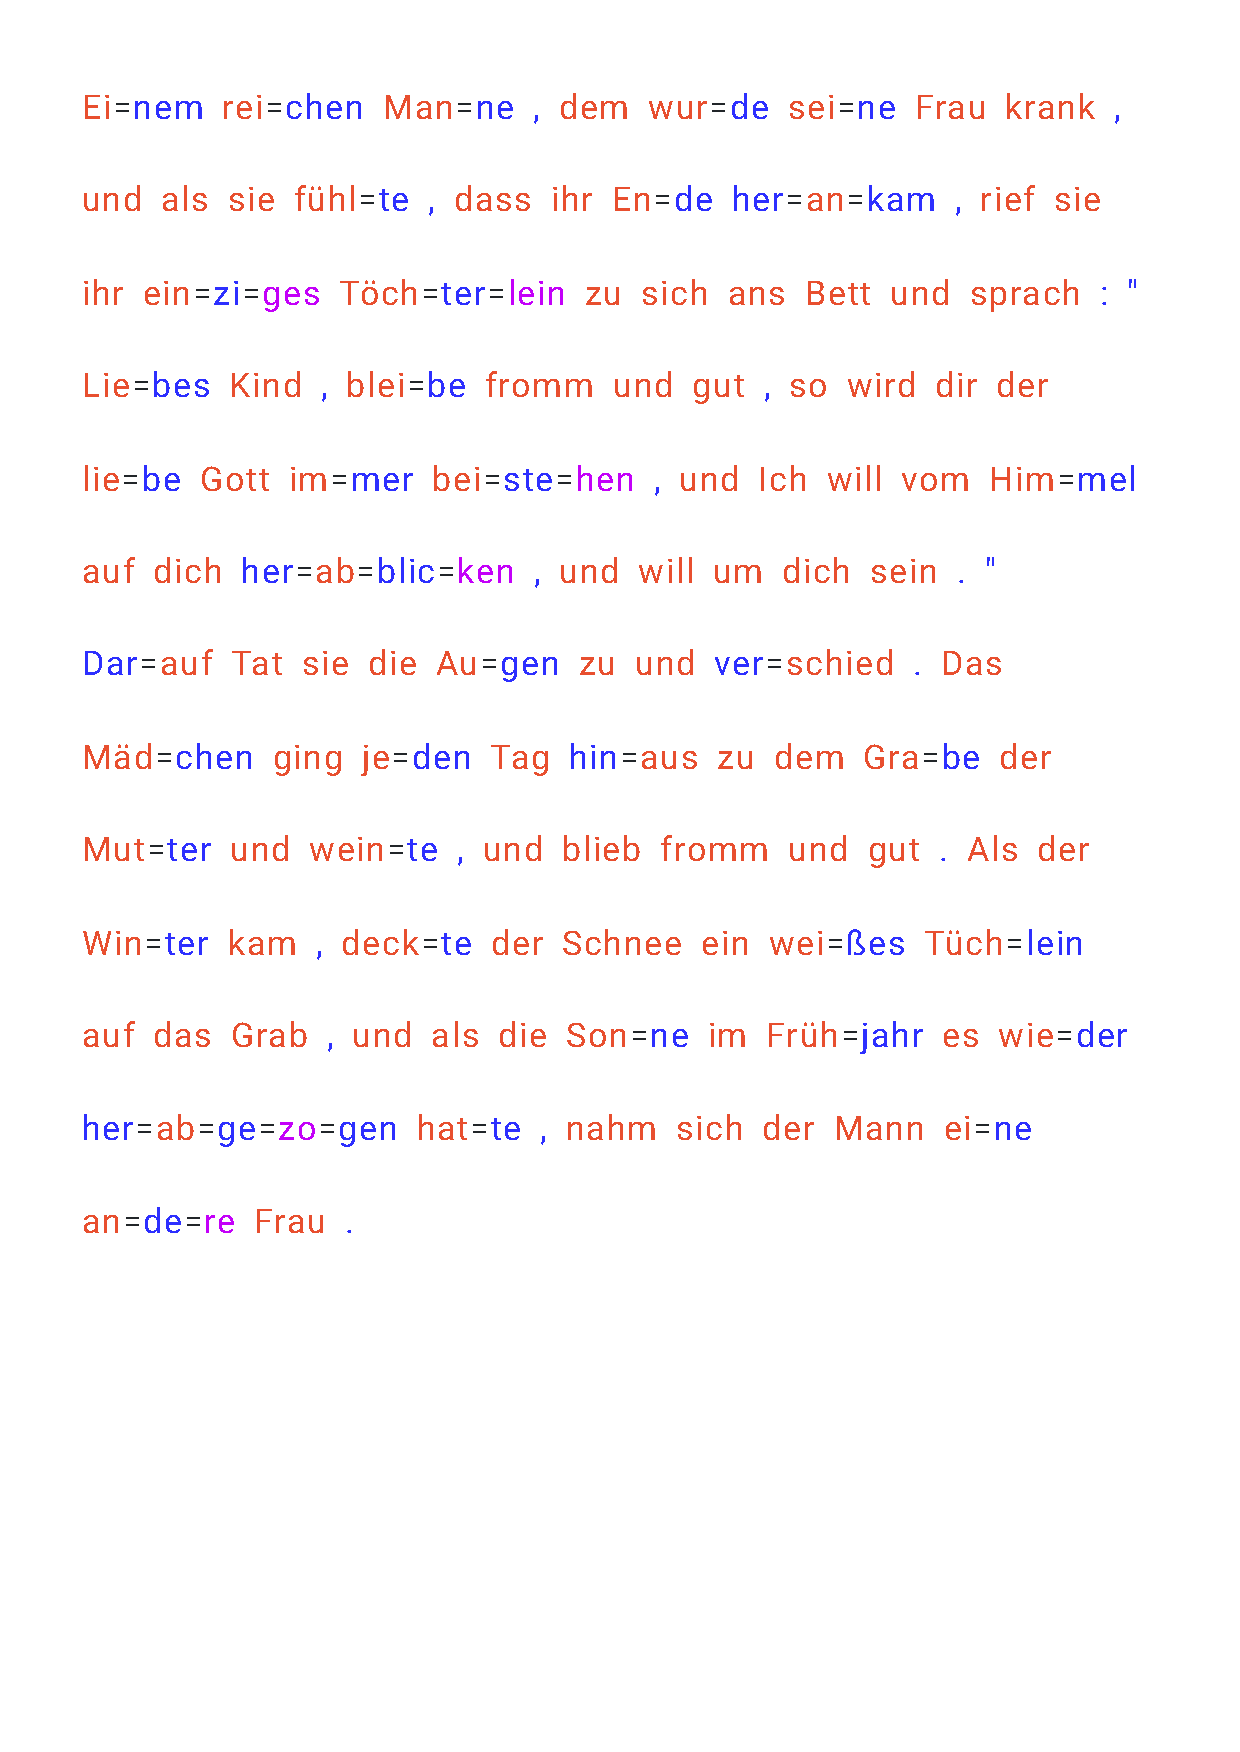
\includegraphics[width=.7\linewidth, frame]{figures/evaluation/annotation3}
	\caption{Silbentrennzeichen und verschiedene Silbenfarben}
	\label{fig:evaluation-ex3}
\end{figure}
\newpage

\subsubsection{Beispiel 4: Hervorhebung des Silbenhintergrunds}

In diesem Beispiel wird ein anderer Ansatz der farblichen Hervorhebung gewählt. Die eingestellten Farben bestimmen hier den Hintergrund der Silben und nicht die Schriftfarbe (diese ist immer Schwarz). Das Beispiel hebt vor Allem die betonte Silbe hervor, die grün dargestellt werden. Unbetonte Silben bekommen alterierend zwei verschiedene Grautöne als Hintergrund. Der Silbenabstand ist hier wieder \textit{0}, somit wird die Einheit des Wortes deutlich erkennbar.

\begin{figure}[h!]
	\centering
	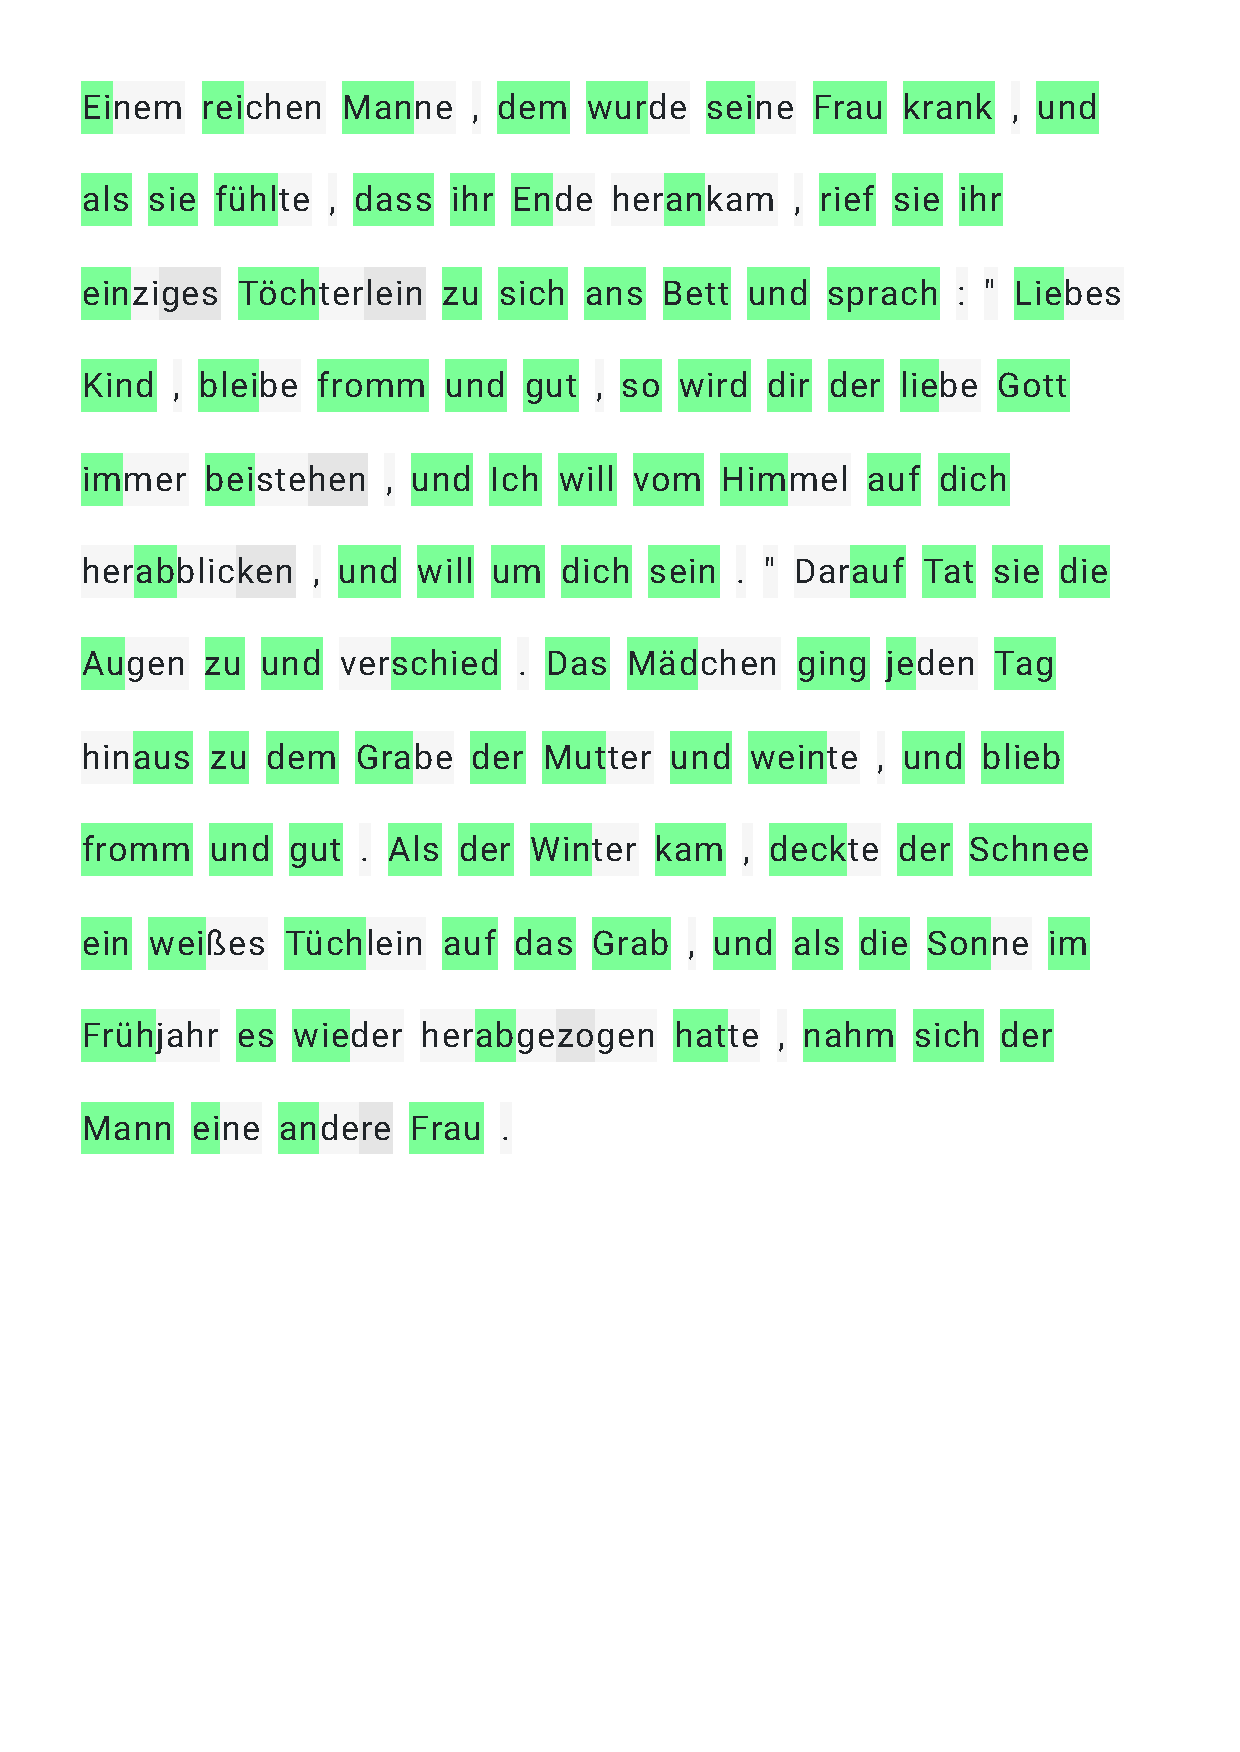
\includegraphics[width=.7\linewidth, frame]{figures/evaluation/annotation4}
	\caption{Hervorhebung des Silbenhintergrunds}
	\label{fig:evaluation-ex4}
\end{figure}
\newpage

\subsubsection{Beispiel 5: Manuelles Deaktivieren der Hervorhebung in kurzen Wörtern}

In Beispiel 5 wird der Sprachrhythmus mit Wortbetonungen noch deutlicher hervorgehoben. Die betonte Silbe wir zusätzlich zur grünen Farbe auch fett dargestellt. Außerdem wurde die Betonung in manchen Wörtern deaktiviert, so werden im ganzen Text beispielsweise Artikel, Präpositionen oder manche einsilbigen Wörter nicht betont markiert. Dieser Text soll damit einen Fokus auf den Sprachrhythmus innerhalb ganzer Sätze legen.

\begin{figure}[h!]
	\centering
	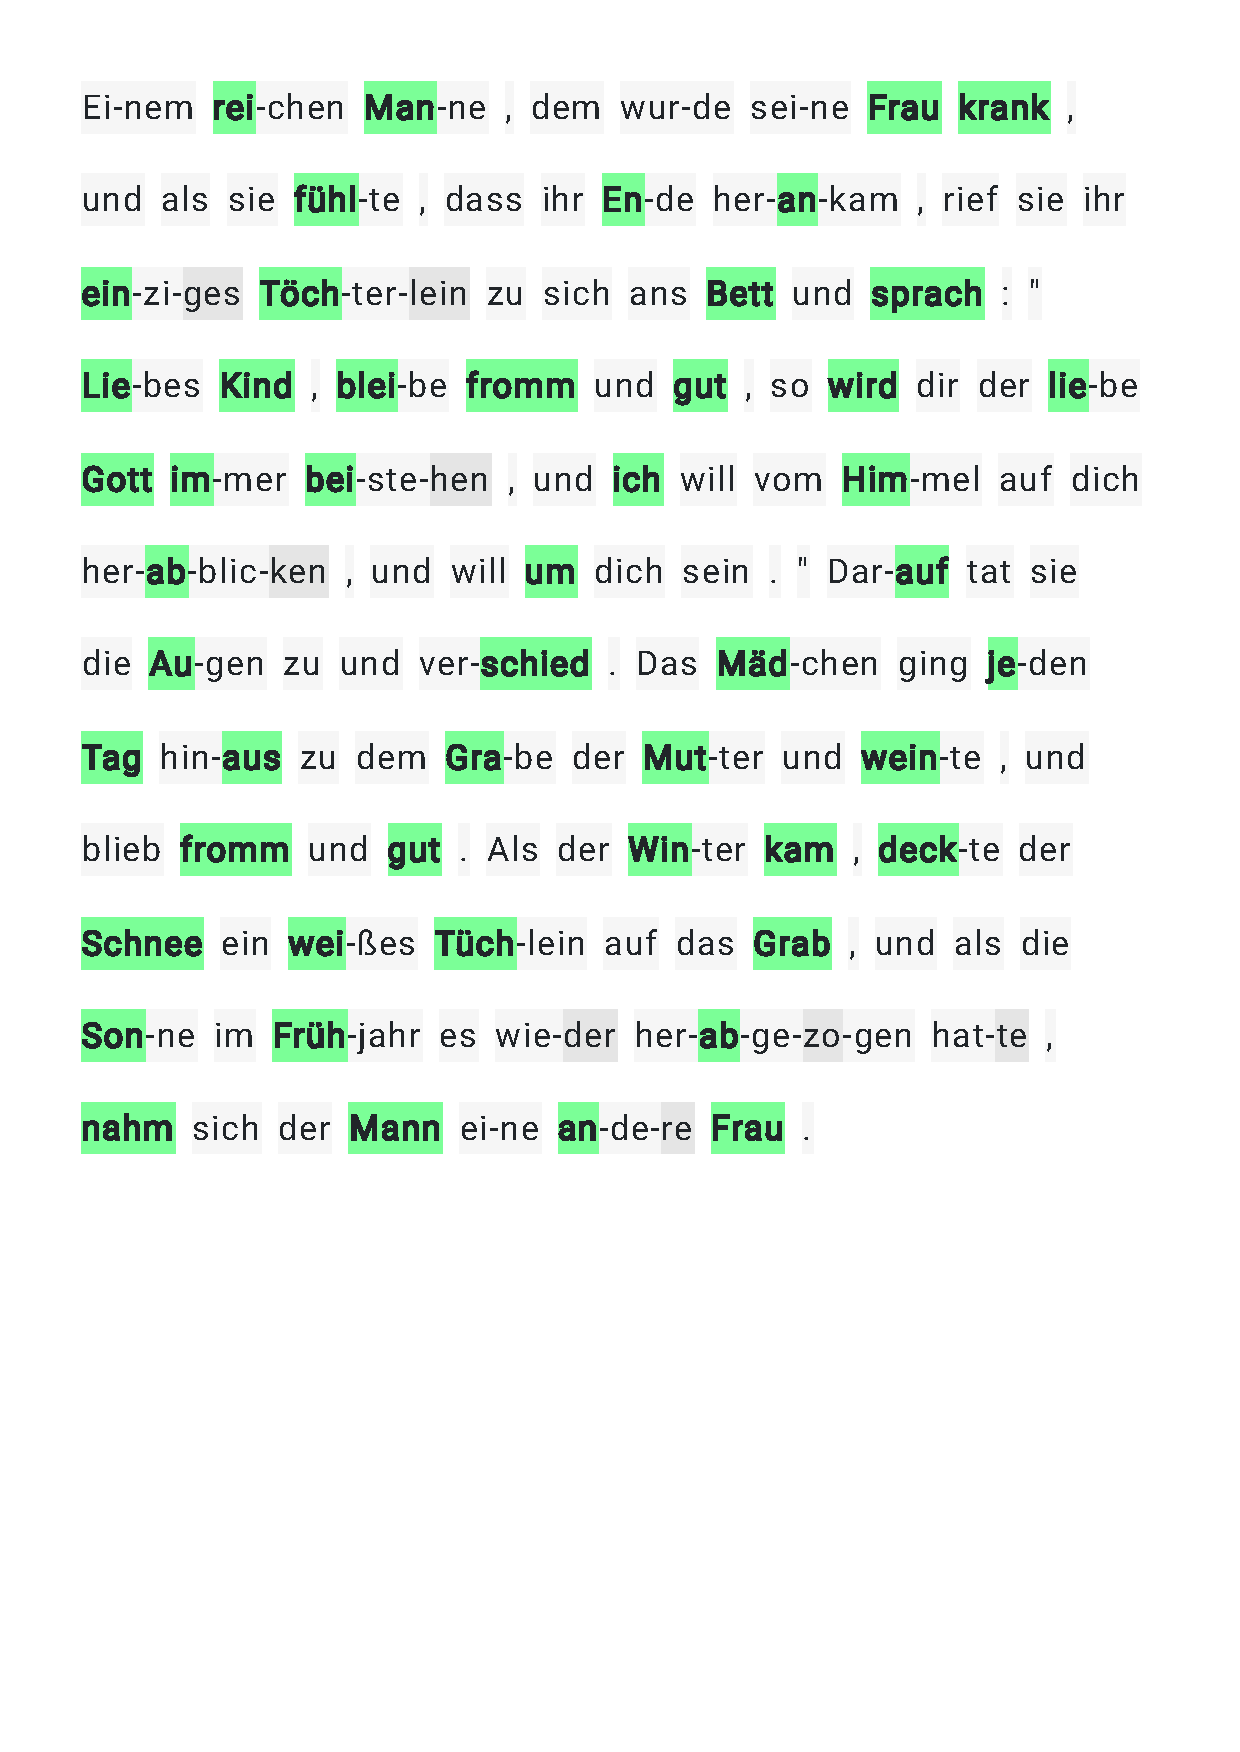
\includegraphics[width=.7\linewidth, frame]{figures/evaluation/annotation5}
	\caption{Manuelles Deaktivieren der Hervorhebung in kurzen Wörtern}
	\label{fig:evaluation-ex5}
\end{figure}
\newpage

\section{Nutzertest}

Während die Beispiele im vorherigen Abschnitt verdeutlichen, dass das Entwickelte Programm generell dazu in der Lage ist, Texte anforderungsgemäß zu annotieren, sollte der Nutzertest zeigen, dass die Applikation von der Zielgruppe (Lerntherapeuten, Nachhilfelehrer und Eltern betroffener Kinder) problemlos bedient werden kann. Intuitivität und Zeiteffizienz sollten dabei vor Allem berücksichtigt werden, da Software, die diese Kriterien schlecht erfüllt, ungern oder im schlechtesten Fall überhaupt nicht benutzt wird. \tocite{irgendwas UX}.

\subsection{Vorbereitung und Durchführung}

Der Nutzertest beinhaltete neben den statistischen Daten zu Alter und Beruf bzw. Studiengang fünf Szenarien, die der Nutzer bearbeiten sollte. Um detaillierte Informationen zur Vorgehensweise des Probanden zu erhalten, wurde im Interview mit der \textit{Thinking Aloud} Methode gearbeitet, d.h. der Proband wurde aufgefordert bei jeder Aktion, die er durchführt, möglichst genau zu beschreiben was er damit bezweckt und warum er es tut. \tocite{thinking aloud} In der schriftlichen Testbeschreibung wurde der Nutzer daher informiert, alle Arbeitsschritte der Szenarien laut vorzulesen und Kommentare und Kritik jederzeit zu äußern. Außerdem wurde in jedem Text explizit mündlich darauf hingewiesen, alle Handlungen möglichst genau zu beschreiben.\\
In der Testbeschreibung wurde auch verdeutlicht, dass es sich um ein Test des Softwaresystems handelt und nicht des Nutzers. \todo{warum wichtic, cite}\\

Um möglichst konsistente Testbedingungen zu schaffen, wurde bei allen Probanden mit einer aktuellen Version von Google Chrome gearbeitet. Es wurde zudem sichergestellt, dass den Probanden ein möglichst gewohntes Umfeld geboten wird. Im besten Fall benutzten die Nutzer ihre eigenen Computer. Falls dies nicht möglich war, wurde vorher überprüft ob beim Testgerät alles genauso wie gewohnt bedient werden konnte, d.h. Einstellungen für Peripherie wie Maus, Tastatur oder Touchpad wurden vorher, dem Nutzer entsprechend, angepasst.\\

Nach jedem der fünf Szenarien wurde von dem Proband ein After Scenario Questionnaire ausgefüllt \tocite{asq}. Es beinhaltete die folgenden drei Fragen:
\begin{itemize}
	\item \textbf{Intuitivität}: Die Aufgabe konnte ich intuitiv und problemlos erledigen.
	\item \textbf{Zeitaufwand}: Ich halte die Zeit, die ich gebraucht habe um die Aufgabe zu erledigen, für angemessen.
	\item \textbf{Dokumentation}: Ich bin mit den Informationen, die ich während der Bearbeitung in der App erhalten habe (Beschreibungen, Rückmeldungen) zufrieden.
\end{itemize}

Zustimmung oder Ablehnung der Aussagen konnte in den fünf Optionen \textit{trifft zu}, \textit{trifft eher zu}, \textit{weder noch}, \textit{trifft eher nicht zu} oder \textit{trifft nicht zu} ausgedrückt werden.

Die Software wurde insgesamt 7 Probanden getestet. Die Bedienung der Software sollte sich im besten Fall möglichst wenig unterscheiden, wenn sie durch Experten oder Laien durchgeführt wird. Daher wurden die Befragten in die entsprechenden zwei Gruppen eingeteilt. Zum einen die Expertengruppe, bestehend aus Lerntherapeuten und Nachhilfelehrern, und zum Anderen Laien, die exemplarisch für Leute aus dem Umfeld der Betroffenen stehen. Es wurden 3 Experten und 4 Laien befragt.\\

\subsection{Ergebnisse}

Im Folgenden werden die einzelnen Szenarien beschrieben und deren Ergebnisse dargestellt. Von den Probanden erkannte und während des Szenarios geäußerte Schwierigkeiten und Probleme werden tabellarisch, zusammen mit eventuellen Ansätzen zu deren Behebung dargestellt.

\subsubsection{Szenario 1: Nutzerkonto}

Zuerst sollte der Proband ein Nutzerkonto mit Mail Adresse und Passwort erstellen (hier wurde, damit der Nutzer kein sicherheitskritisches Passwort verwendet und sich das Passwort während des Tests merken kann \qq{12345678} vorgegeben). Anschließend loggt er sich ein und wieder aus.

\begin{figure}[h!]
	\centering
	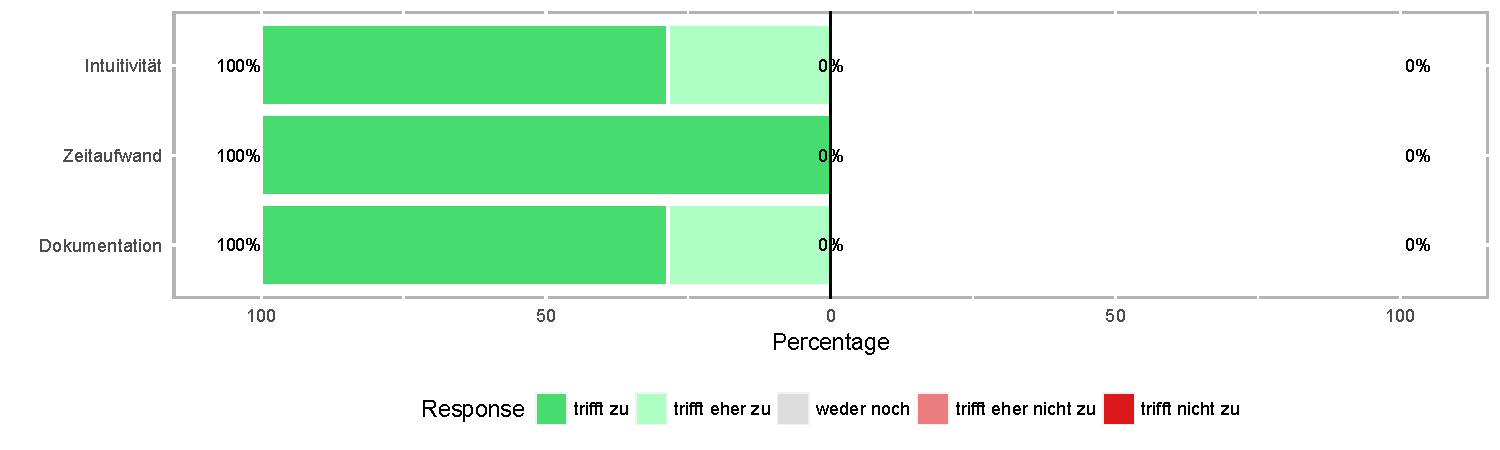
\includegraphics[width=.8\linewidth]{figures/evaluation/scenario1}
	\caption{Quantitative Ergebnisse von Szenario 1 (Nutzerkonto)}
	\label{fig:evaluation-sc1}
\end{figure}

Die Testpersonen konnten die Aufgabe meist problemlos lösen. Mehrmals wurde vor dem Erstellen des neuen Kontos erst Email Adresse und Passwort in das Login Fenster eingetragen, was zu einer Fehlermeldung führte (da das Konto noch nicht existiert). Die Testpersonen kamen aber in jedem Fall selbst darauf, dass man dem Link \textit{Neues Konto erstellen folgen} musste. Hier könnte die Unterscheidung zwischen Login und Konto erstellen noch deutlicher gemacht werden bzw. könnte der Link zum Konto erstellen besser sichtbar platziert werden (s. Tabelle \ref{table:szenario1} im Anhang).

\subsubsection{Szenario 2: Textanalyse}

Als nächstes loggt sich der Proband wieder ein und soll einen gegebenen Text in das Textfeld der Textanalyse kopieren und diesen dann analysieren lassen. Alle unbekannten Wörter (in der Anwendung rot hinterlegt) sollen nun manuell geklärt werden. Der Nutzer klickt so lange durch das User Interface der manuellen Analyse, bis alle Wörter annotiert sind. Als letztes soll mit den Einstellungen der Annotation experimentiert werden, bis eine Einstellung gefunden wird, die den Nutzer anspricht. Hier wurde noch mündlich hinzugefügt, dass der Nutzer, um sich damit vertraut zu machen, alle Einstellungen einmal ausprobieren sollte.

\begin{figure}[h!]
	\centering
	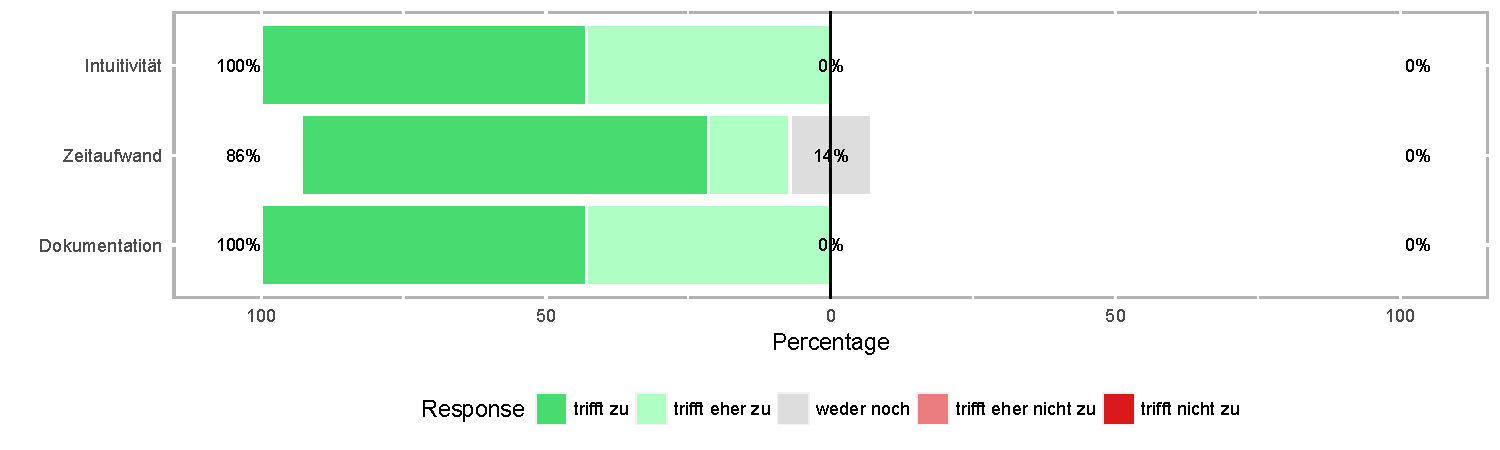
\includegraphics[width=.8\linewidth]{figures/evaluation/scenario2}
	\caption{Quantitative Ergebnisse von Szenario 2 (Textanalyse)}
	\label{fig:evaluation-sc2}
\end{figure}

Auch hier konnten alle Testpersonen die Aufgabe bewältigen. Es wurde teilweise das Layout bemängelt. Es war umständlich, Einstellungen zu verändern, wenn man dafür weit runter scrollen musste und so den Vorschautext nicht mehr im Blick hatte. Hier wurde eine kompaktere Darstellung der Einstellungen gewünscht. Es wurde außerdem vorgeschlagen, die Farbauswahl zu vereinfachen, sodass dafür nicht jedes mal ein extra Fenster aufgeht (s. Tabelle \ref{table:szenario2} im Anhang).

\subsubsection{Szenario 3: Annotationsvorlagen}

Im dritten Szenario werden dem Nutzer zweimal die erste Zeile des Textes, jeweils mit verschieden Einstellungen annotiert, gegeben. Er soll nun nacheinander versuchen, die Annotation so einzustellen, dass es so wie im gegebenen Ausschnitt aussieht. Zudem sollen diese Einstellungen als Vorlagen mit den Namen \qq{Vorlage 1} und \qq{Vorlage 2} gespeichert werden. Zum Schluss wechselt der Nutzer zwischen Vorlage 1 und Vorlage 2 hin und her.

\begin{figure}[h!]
	\centering
	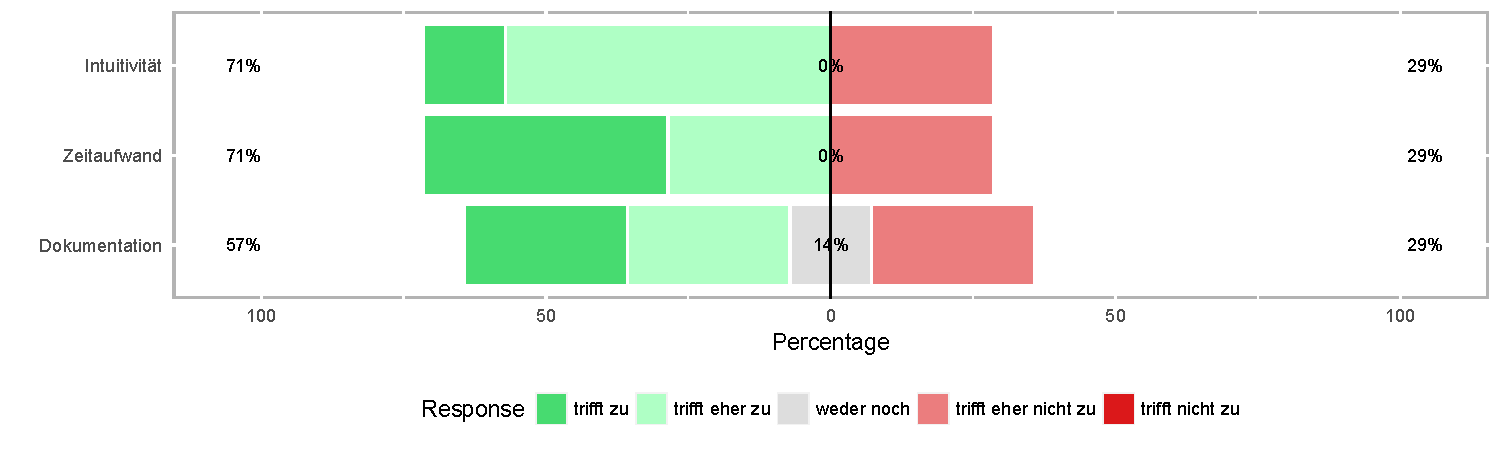
\includegraphics[width=.8\linewidth]{figures/evaluation/scenario3}
	\caption{Quantitative Ergebnisse von Szenario 3 (Annotationsvorlagen)}
	\label{fig:evaluation-sc3}
\end{figure}

Das Speichern und Wechseln der Vorlagen bereitete den Testpersonen hier großteils keine Probleme. Fast alle Nutzerinnen und Nutzer konnten allerdings den Text für Vorlage 2 (farbiger Hintergrund mit schwarzer Schrift) nicht ohne Hilfe entsprechend anpassen. Hier war nicht klar, was die Option \textit{Silbe betonen} bedeutete und wurde oft mit der \textit{Wort Hintergrundfarbe} verwechselt. Erst durch längeres ausprobieren oder Hilfestellungen konnten die Testpersonen die Aufgabe lösen. Hier sollte zum Einen der Aufbau und die Beschreibung der Elemente der Einstellungen überarbeitet werden, zum Anderen legen die Probleme bei den Einstellungen nahe, eine kurze Einführung (evtl. in Form einer Kurzdokumentation oder Online-Hilfe in der Applikation) bereitzustellen (s. Tabelle \ref{table:szenario3} im Anhang).

\subsubsection{Szenario 4: Texte wiederverwenden}

Hier soll der Nutzer den aktuellen Text mit Titel in seinem Nutzerkonto speichern. Anschließen wird auf die Nutzerkonto Seite gewechselt und der gespeicherte Text neu analysiert.

\begin{figure}[h!]
	\centering
	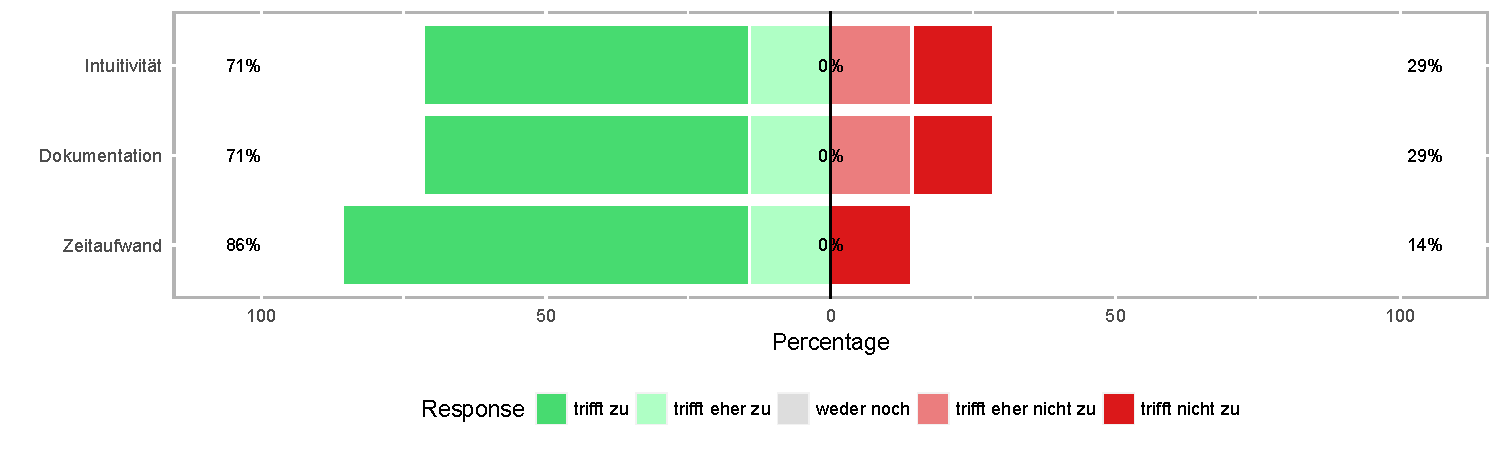
\includegraphics[width=.8\linewidth]{figures/evaluation/scenario4}
	\caption{Quantitative Ergebnisse von Szenario 4 (Texte wiederverwenden)}
	\label{fig:evaluation-sc4}
\end{figure}

Die meisten Testpersonen konnten diese Aufgabestellung problemlos lösen. Zwei Probandinnen konnten die Aufgabe allerdings nicht ohne Hilfestellung bewältigen, da die Nutzerseite nicht gefunden wurde. Hier war nicht klar, dass der Link rechts oben in der Navigation zur Nutzerkonto Seite führt und dort Nutzertexte gespeichert sind. Die Navigation könnte hier noch deutlicher und übersichtlicher gestaltet werden (s. Tabelle \ref{table:szenario4} im Anhang).

\subsubsection{Szenario 5: Wort Verifizierung}

Im letzten Szenario wechselt der Nutzer auf die Verifizierungsseite. Hier sollen vier Einträge anderer Nutzer bestätigt oder verbessert werden.

\begin{figure}[h!]
	\centering
	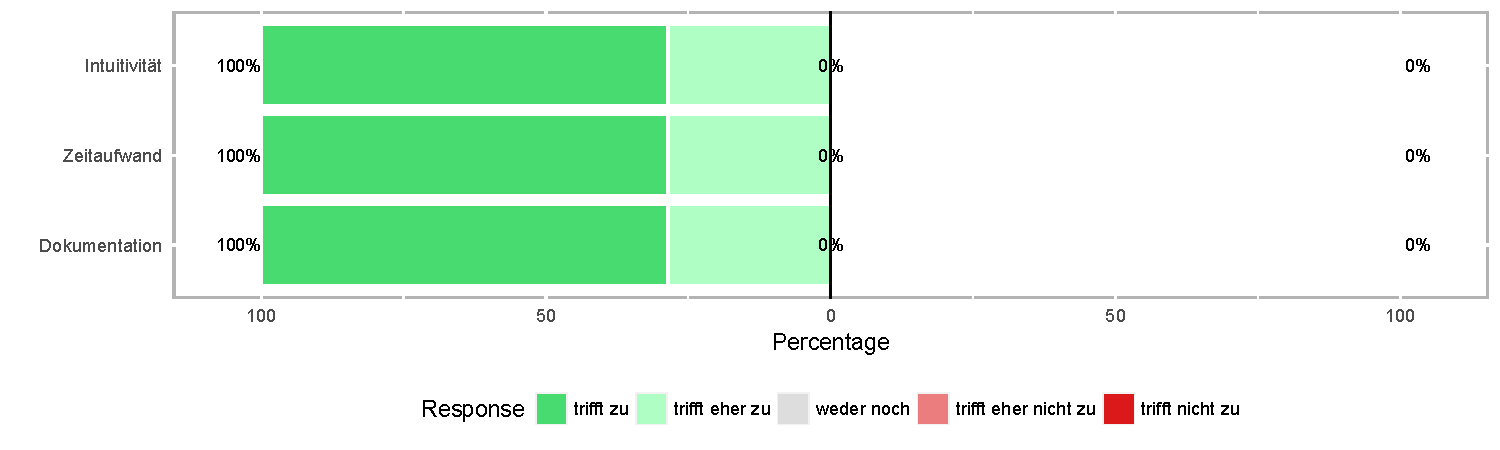
\includegraphics[width=.8\linewidth]{figures/evaluation/scenario5}
	\caption{Quantitative Ergebnisse von Szenario 5 (Wort Verifizierung)}
	\label{fig:evaluation-sc5}
\end{figure}

Bei der Durchführung der Verifizierung gab es keine größeren Probleme. In einigen Vorschläge bemerkten die Testpersonen, dass der Prozess zum Beispiel verbessert werden könnten, indem mehrere Wörter auf einmal in einer Liste \qq{abgehakt} werden könnten oder für Änderungen bei der Segmentierung die Texteingabe für die Silbentrennung vereinfacht werden könnte (s. Tabelle \ref{table:szenario5} im Anhang).

\subsubsection{Allgemeine Anmerkungen}

Zum Schluss des Nutzertest wurde die Probandinnen und Probanden zu allgemeinen Äußerungen von Kritik und Vorschlägen zur Applikation als Ganzes aufgefordert. Wichtige Ideen und Kommentare sind im Folgenden festgehalten:

\begin{itemize}
	\item Alte, nicht mehr aktuelle Fehlermeldungen verschwinden oft nicht (oder nur, wenn man sie selbst schließt). Diese sollten sich beim Ausführen neuer Interaktionen automatisch schließen.
	\item Die \textit{Home} Seite sollte die Beschreibungen besser gruppieren (z.B. nebeneinander mit Bildern) und die Breite besser ausnutzen.
	\item Die türkise Farbe für die Umrandung der Kästen wirkte unpassend. Diese könnte in die blaue Farbe der Links geändert werden.
	\item Es wurde eine Option gewünscht, bei der die Wortbetonung in der Annotation vollständig ausgeschaltet wird und stattdessen ein einfaches, abwechselndes Einfärben der Silben (über Wortgrenzen hinaus) ermöglicht wird.
	\item Beim Navi-Link zum Nutzerkonto (Email Adresse rechts oben) könnte ein Bücherregal Symbol verdeutlichen, dass dort Nutzertexte zur Wiederverwendung gespeichert werden.
\end{itemize}

\newpage
\section{Diskussion}

hat funktioniert\\
wurde von lerntherapeuten als nütlich bewertet, im verglich zur manuellen erstellung der texte\\
usability zeigt, das das programm grunsätzlich gut benutzbar ist, teilweise kleine änderungen nötig, damit für alle problemlos bedienbar\\
teile (wie nur eine betonung im wort) funktionieren, könnten aber noch deutlich besser gemacht/überarbeitet werden\\

einleitung aufgreifen, welche fragen, antworten dazu aus hauptteil und evaluation\\
irgendwelche fragen aus literatur beantwortet?
weitere fragen?

\section{Ausblick}

datenbank: PHONOLEX als Grundlage (statt oder zusaetzlich zu CELEX)\\
welche grundlegenden ideen können noch umgesetzt werden, wie kann die software erweitert werden?\\

falsche einträge in wortdatenbank müssen verbessert werden bzw. fehler melden funktion\\